\documentclass[tikz,border=3pt]{standalone}
\usepackage[T1]{fontenc}
\usepackage[scaled=0.92]{helvet}
\renewcommand{\familydefault}{\sfdefault}
\usepackage{amsmath}
\usetikzlibrary{arrows.meta,positioning,calc,fit,backgrounds,decorations.pathreplacing}

\definecolor{ink}{HTML}{27313D}
\definecolor{muted}{HTML}{5F6C79}
\definecolor{grid}{HTML}{D7DCE2}
\definecolor{gold}{HTML}{F2C66D}
\definecolor{goldline}{HTML}{C98A20}
\definecolor{direct}{HTML}{3569AD}
\definecolor{directlight}{HTML}{EAF1F9}
\definecolor{cot}{HTML}{347E68}
\definecolor{cotlight}{HTML}{E8F3EF}
\definecolor{transition}{HTML}{7154B3}
\definecolor{transitionlight}{HTML}{F0EBF8}
\definecolor{intervention}{HTML}{C5652A}
\definecolor{interventionlight}{HTML}{F9EEE7}
\definecolor{errorred}{HTML}{B24747}
\definecolor{errorlight}{HTML}{F8EDED}

\tikzset{
  >=Latex,
  panel/.style={draw=grid, rounded corners=2.5pt, line width=.75pt, fill=white},
  lane/.style={rounded corners=2.5pt, line width=.65pt},
  nodebase/.style={rounded corners=2pt, line width=.8pt, align=center, inner sep=3pt,
                   font=\fontsize{7.4}{8.4}\selectfont},
  tinylabel/.style={font=\fontsize{6.3}{7.2}\selectfont, text=muted, align=center},
  smalllabel/.style={font=\fontsize{7.2}{8.2}\selectfont, text=ink, align=center},
  title/.style={font=\bfseries\fontsize{9.4}{10.5}\selectfont, text=ink, anchor=west},
  subtitle/.style={font=\fontsize{6.8}{7.8}\selectfont, text=muted, anchor=west},
  flow/.style={-Latex, line width=1pt, draw=ink},
  hypoth/.style={-Latex, dashed, line width=.85pt, draw=muted},
  interventionmark/.style={circle, draw=intervention, fill=white, text=intervention,
                           font=\bfseries\fontsize{6.8}{7.5}\selectfont,
                           minimum size=4.6mm, inner sep=0pt}
}

\begin{document}
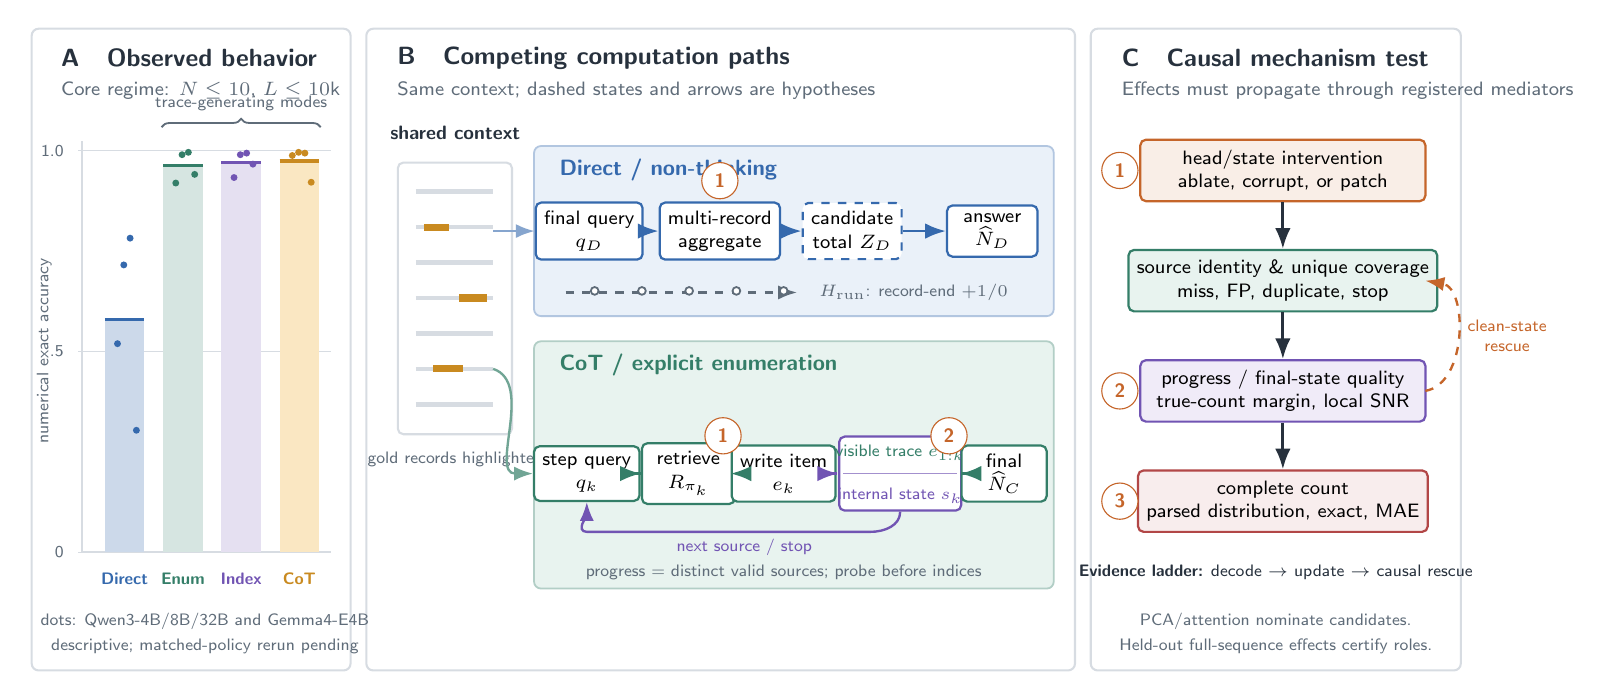
\begin{tikzpicture}[x=1cm,y=1cm]

% Panel backgrounds
\draw[panel] (0,0) rectangle (4.05,8.15);
\draw[panel] (4.25,0) rectangle (13.25,8.15);
\draw[panel] (13.45,0) rectangle (18.15,8.15);

% --------------------------------------------------------------------------
% Panel A: preliminary observed gap
\node[title] at (0.25,7.78) {\textbf{A}\quad Observed behavior};
\node[subtitle] at (0.25,7.36) {Core regime: $N\leq10$, $L\leq10$k};

% axes
\draw[grid,line width=.65pt] (0.64,1.50) -- (0.64,6.72);
\draw[grid,line width=.65pt] (0.64,1.50) -- (3.80,1.50);
\foreach \yy/\lab in {1.50/0,4.05/.5,6.60/1.0}{
  \draw[grid,line width=.45pt] (0.59,\yy) -- (3.80,\yy);
  \node[font=\fontsize{6.2}{7}\selectfont,text=muted,anchor=east] at (0.53,\yy) {\lab};
}
\node[font=\fontsize{6.2}{7}\selectfont,text=muted,rotate=90] at (0.16,4.06) {numerical exact accuracy};

% bars: means across Qwen3-4B/8B/32B and Gemma4-E4B
\path[fill=direct!25] (0.93,1.50) rectangle (1.43,4.46);
\path[fill=cot!20] (1.67,1.50) rectangle (2.17,6.41);
\path[fill=transition!18] (2.41,1.50) rectangle (2.91,6.45);
\path[fill=gold!42] (3.15,1.50) rectangle (3.65,6.47);
\draw[direct,line width=1.15pt] (0.93,4.46) -- (1.43,4.46);
\draw[cot,line width=1.15pt] (1.67,6.41) -- (2.17,6.41);
\draw[transition,line width=1.15pt] (2.41,6.45) -- (2.91,6.45);
\draw[goldline,line width=1.15pt] (3.15,6.47) -- (3.65,6.47);

% individual model dots
\foreach \x/\v in {1.09/4.15,1.17/5.15,1.25/5.49,1.33/3.05}
  \fill[direct] (\x,\v) circle (1.25pt);
\foreach \x/\v in {1.83/6.19,1.91/6.55,1.99/6.58,2.07/6.30}
  \fill[cot] (\x,\v) circle (1.25pt);
\foreach \x/\v in {2.57/6.26,2.65/6.55,2.73/6.57,2.81/6.43}
  \fill[transition] (\x,\v) circle (1.25pt);
\foreach \x/\v in {3.31/6.54,3.39/6.58,3.47/6.57,3.55/6.20}
  \fill[goldline] (\x,\v) circle (1.25pt);

\node[font=\bfseries\fontsize{6.4}{7.2}\selectfont,text=direct] at (1.18,1.16) {Direct};
\node[font=\bfseries\fontsize{6.4}{7.2}\selectfont,text=cot] at (1.92,1.16) {Enum};
\node[font=\bfseries\fontsize{6.4}{7.2}\selectfont,text=transition] at (2.66,1.16) {Index};
\node[font=\bfseries\fontsize{6.4}{7.2}\selectfont,text=goldline] at (3.40,1.16) {CoT};
\draw[decorate,decoration={brace,amplitude=3pt},muted,line width=.65pt]
  (1.65,6.90) -- (3.67,6.90);
\node[tinylabel,anchor=south] at (2.66,6.98) {trace-generating modes};
\node[tinylabel] at (2.20,.62) {dots: Qwen3-4B/8B/32B and Gemma4-E4B};
\node[tinylabel] at (2.20,.30) {descriptive; matched-policy rerun pending};

% --------------------------------------------------------------------------
% Panel B: computation paths
\node[title] at (4.52,7.78) {\textbf{B}\quad Competing computation paths};
\node[subtitle] at (4.52,7.36) {Same context; dashed states and arrows are hypotheses};

% shared context
\node[smalllabel,font=\bfseries\fontsize{7.2}{8.2}\selectfont] at (5.38,6.83) {shared context};
\draw[rounded corners=2pt,draw=grid,fill=white,line width=.75pt] (4.65,3.00) rectangle (6.10,6.45);
\foreach \yy in {3.38,3.83,4.28,4.73,5.18,5.63,6.08}{
  \draw[grid,line width=1.7pt] (4.88,\yy) -- (5.86,\yy);
}
\draw[goldline,line width=2.6pt] (5.10,3.83) -- (5.48,3.83);
\draw[goldline,line width=2.6pt] (5.43,4.73) -- (5.78,4.73);
\draw[goldline,line width=2.6pt] (4.98,5.63) -- (5.30,5.63);
\node[tinylabel] at (5.38,2.68) {gold records highlighted};

% lane backgrounds
\draw[lane,draw=direct!38,fill=directlight] (6.38,4.50) rectangle (12.98,6.66);
\draw[lane,draw=cot!38,fill=cotlight] (6.38,1.04) rectangle (12.98,4.18);
\node[font=\bfseries\fontsize{7.8}{8.8}\selectfont,text=direct,anchor=west] at (6.58,6.36)
  {Direct / non-thinking};
\node[font=\bfseries\fontsize{7.8}{8.8}\selectfont,text=cot,anchor=west] at (6.58,3.88)
  {CoT / explicit enumeration};

% Direct lane nodes and fan-in
\node[nodebase,draw=direct,fill=white,minimum width=1.16cm] (qd) at (7.08,5.58) {final query\\$q_D$};
\node[nodebase,draw=direct,fill=white,minimum width=1.45cm] (agg) at (8.74,5.58) {multi-record\\aggregate};
\node[nodebase,draw=direct,dashed,fill=white,minimum width=1.18cm] (zd) at (10.42,5.58) {candidate\\total $Z_D$};
\node[nodebase,draw=direct,fill=white,minimum width=1.15cm] (ad) at (12.20,5.58) {answer\\$\widehat N_D$};
\draw[flow,draw=direct] (qd) -- (agg);
\draw[flow,draw=direct] (agg) -- (zd);
\draw[flow,draw=direct] (zd) -- (ad);
\draw[-Latex,draw=direct!60,line width=.85pt] (5.86,5.58) -- (qd.west);

% Direct competing running-state hypothesis
\draw[hypoth] (6.78,4.80) -- (9.72,4.80);
\foreach \xx in {7.15,7.75,8.35,8.95,9.55}{
  \draw[draw=muted,fill=white,line width=.65pt] (\xx,4.82) circle (1.4pt);
}
\node[tinylabel,anchor=west] at (9.88,4.80) {$H_{\rm run}$: record-end $+1/0$};
\node[interventionmark] at (8.74,6.22) {1};

% CoT lane nodes
\node[nodebase,draw=cot,fill=white,minimum width=1.04cm] (qk) at (7.05,2.50) {step query\\$q_k$};
\node[nodebase,draw=cot,fill=white,minimum width=1.18cm] (ret) at (8.34,2.50) {retrieve\\$R_{\pi_k}$};
\node[nodebase,draw=cot,fill=white,minimum width=1.05cm] (ek) at (9.55,2.50) {write item\\$e_k$};
\node[nodebase,draw=transition,fill=white,minimum width=1.55cm,minimum height=.94cm] (gamma) at (11.03,2.50) {};
\draw[transition!65,line width=.55pt] (10.31,2.50) -- (11.75,2.50);
\node[font=\fontsize{6.5}{7.3}\selectfont,text=cot] at (11.03,2.77) {visible trace $e_{1:k}$};
\node[font=\fontsize{6.5}{7.3}\selectfont,text=transition] at (11.03,2.22) {internal state $s_k$};
\node[nodebase,draw=cot,fill=white,minimum width=1.08cm] (ac) at (12.35,2.50) {final\\$\widehat N_C$};
\draw[flow,draw=cot] (qk) -- (ret);
\draw[flow,draw=cot] (ret) -- (ek);
\draw[flow,draw=transition] (ek) -- (gamma);
\draw[flow,draw=cot] (gamma) -- (ac);
\draw[-Latex,draw=cot!70,line width=.85pt] (5.86,3.83)
  to[out=-18,in=180] (qk.west);
\draw[-Latex,draw=transition,line width=.85pt] (gamma.south)
  to[out=-90,in=0] (10.65,1.76) -- (7.05,1.76)
  to[out=180,in=-90] (qk.south);
\node[interventionmark] at (8.78,2.98) {1};
\node[interventionmark] at (11.65,2.98) {2};
\node[tinylabel,text=transition] at (9.05,1.56) {next source / stop};
\node[tinylabel] at (9.55,1.24) {progress = distinct valid sources; probe before indices};

% --------------------------------------------------------------------------
% Panel C: integrated causal chain
\node[title] at (13.72,7.78) {\textbf{C}\quad Causal mechanism test};
\node[subtitle] at (13.72,7.36) {Effects must propagate through registered mediators};

\node[nodebase,draw=intervention,fill=interventionlight,minimum width=3.62cm,minimum height=.78cm]
  (int) at (15.89,6.35) {head/state intervention\\ablate, corrupt, or patch};
\node[nodebase,draw=cot,fill=cotlight,minimum width=3.62cm,minimum height=.78cm]
  (ident) at (15.89,4.95) {source identity \& unique coverage\\miss, FP, duplicate, stop};
\node[nodebase,draw=transition,fill=transitionlight,minimum width=3.62cm,minimum height=.78cm]
  (state) at (15.89,3.55) {progress / final-state quality\\true-count margin, local SNR};
\node[nodebase,draw=errorred,fill=errorlight,minimum width=3.62cm,minimum height=.78cm]
  (err) at (15.89,2.15) {complete count\\parsed distribution, exact, MAE};
\draw[flow] (int) -- (ident);
\draw[flow] (ident) -- (state);
\draw[flow] (state) -- (err);
\node[interventionmark] at (13.82,6.35) {1};
\node[interventionmark] at (13.82,3.55) {2};
\node[interventionmark] at (13.82,2.15) {3};

\draw[hypoth,draw=intervention] (17.70,3.55) to[out=10,in=-10]
  node[tinylabel,right,text=intervention] {clean-state\\rescue} (17.70,4.95);
\node[tinylabel,text=ink] at (15.80,1.25) {\textbf{Evidence ladder:} decode $\rightarrow$ update $\rightarrow$ causal rescue};
\node[tinylabel] at (15.80,.62) {PCA/attention nominate candidates.};
\node[tinylabel] at (15.80,.30) {Held-out full-sequence effects certify roles.};

\end{tikzpicture}
\end{document}
